\documentclass[11pt,a4paper,twoside,openright]{book}

% ===== LANGUAGE AND ENCODING =====
\usepackage[utf8]{inputenc}
\usepackage[T1]{fontenc}
\usepackage[english]{babel}

% ===== FONTS =====
\usepackage{lmodern}
\usepackage{microtype}

% ===== MATH =====
\usepackage{amsmath}
\usepackage{amssymb}
\usepackage{mathtools}
\usepackage{bm}

% ===== FIGURES =====
\usepackage{graphicx}
\usepackage{float}
\usepackage[font=small,labelfont=bf]{caption}
\usepackage{subcaption}
\graphicspath{{Graphics/}}   % put all images in a figures/ subfolder

% ===== TABLES =====
\usepackage{booktabs}
\usepackage{array}
\usepackage{multirow}

% ===== CODE LISTINGS =====
\usepackage{listings}
\usepackage{xcolor}

\definecolor{codegreen}{rgb}{0,0.6,0}
\definecolor{codegray}{rgb}{0.5,0.5,0.5}
\definecolor{codepurple}{rgb}{0.58,0,0.82}
\definecolor{backcolour}{rgb}{0.97,0.97,0.97}

\lstdefinestyle{mystyle}{
    backgroundcolor=\color{backcolour},
    commentstyle=\color{codegreen},
    keywordstyle=\color{blue}\bfseries,
    numberstyle=\tiny\color{codegray},
    stringstyle=\color{codepurple},
    basicstyle=\ttfamily\footnotesize,
    breaklines=true,
    captionpos=b,
    keepspaces=true,
    numbers=left,
    numbersep=8pt,
    frame=single,
    framerule=0.5pt,
    rulecolor=\color{black!30}
}
\lstset{style=mystyle}

% ===== BIBLIOGRAPHY =====
\usepackage{csquotes}
\usepackage[
  backend=biber,
  style=ieee,
  sorting=none,
  maxbibnames=99
]{biblatex}
\addbibresource{references.bib}  % <-- update path if needed

% ===== PAGE GEOMETRY =====
\usepackage[
  inner=3cm,
  outer=2.5cm,
  top=2.5cm,
  bottom=3cm,
  headheight=14pt
]{geometry}

% ===== HEADERS AND FOOTERS =====
\usepackage{fancyhdr}
\pagestyle{fancy}
\fancyhf{}
\fancyhead[LE]{\nouppercase{\leftmark}}
\fancyhead[RO]{\nouppercase{\rightmark}}
\fancyfoot[C]{\thepage}
\renewcommand{\headrulewidth}{0.4pt}

\fancypagestyle{plain}{
  \fancyhf{}
  \fancyfoot[C]{\thepage}
  \renewcommand{\headrulewidth}{0pt}
}

% ===== CHAPTER STYLING =====
\usepackage{titlesec}
\titleformat{\chapter}[display]
  {\normalfont\huge\bfseries}{\chaptertitlename\ \thechapter}{20pt}{\Huge}
\titlespacing*{\chapter}{0pt}{0pt}{40pt}

% ===== LINE SPACING =====
\usepackage{setspace}
\onehalfspacing

% ===== TABLE OF CONTENTS STYLING =====
\usepackage{tocloft}
\renewcommand{\cftchapfont}{\bfseries}
\renewcommand{\cftchappagefont}{\bfseries}

% ===== HYPERLINKS =====
\usepackage[
  colorlinks=true,
  linkcolor=black,
  citecolor=blue,
  urlcolor=blue,
  bookmarks=true,
  bookmarksnumbered=true,
  pdfstartview=FitH,
  pdftitle={Thesis_OskarDeClerck_2026},   % <-- update
  pdfauthor={Oskar De Clerck}
]{hyperref}

% ===== CUSTOM COMMANDS =====
% Bold paragraph heading that does NOT appear in the ToC
\newcommand{\smalltitle}[1]{%
  \vspace{0.5cm}%
  \noindent\textbf{#1}%
  \vspace{0.2cm}%
  \par\noindent%
}

% To erase space between list items.
\usepackage{enumitem}

% ===== DOCUMENT METADATA =====
\title{Robotic Testbench for Collaborative Handling of Payloads with Varying Weights using Compliant Joint Transmissions}
\author{Oskar De Clerck}
\date{May 2026}


% ============================================================
\begin{document}
% ============================================================

% ===== TITLE PAGE =====
\begin{titlepage}
    \centering
    \vspace*{2cm}

    {\Large\scshape KU Leuven\par}
    \vspace{0.5cm}
    {\large Faculty of Engineering Technology\par}
    \vspace{2.5cm}

    {\Huge\bfseries Your Thesis Title Here\par}   % <-- update
    \vspace{0.5cm}
    \rule{10cm}{0.4pt}\par
    \vspace{3cm}

    {\Large\itshape Oskar De Clerck\par}
    \vfill

    {\large A thesis submitted for the degree of\\
    Master of Science in \textit{industriële wetenschappen: Elektromechanica}\par}
    \vfill

    {\large Academic Year 2025--2026\par}
    \vspace{0.5cm}
    {\large Promotor: ir.\ Maurizio Grossi\par}
    {\large Copromotor: prof.\ dr.\ ir.\ Dino Accoto\par}
\end{titlepage}


% ============================================================
%  FRONT MATTER
% ============================================================
\frontmatter

\chapter*{Abstract}
\addcontentsline{toc}{chapter}{Abstract}
% Write last. ~300-500 words.
\cleardoublepage

\chapter*{Acknowledgements}
\addcontentsline{toc}{chapter}{Acknowledgements}
\cleardoublepage

\tableofcontents
\cleardoublepage

\listoffigures
\cleardoublepage

\listoftables
\cleardoublepage

\chapter*{Nomenclature}
\addcontentsline{toc}{chapter}{Nomenclature}

\section*{Symbols}
\begin{tabular}{@{}lll@{}}
  $\bm{q}$    & Joint position vector  & [rad]    \\
  $K_s$       & Spring stiffness       & [Nm/rad] \\
  % add rows here
\end{tabular}

\vspace{1cm}
\section*{Abbreviations}
\begin{tabular}{@{}ll@{}}
  CAN  & Controller Area Network \\
  SET  & Series Elastic Transmission \\
  % add rows here
\end{tabular}

\cleardoublepage


% ============================================================
%  MAIN MATTER
% ============================================================
\mainmatter

% ============================================================
\chapter{Introduction}
\label{ch:introduction}
% ============================================================

\section{Background and Motivation}

\subsection{Musculoskeletal disorders and ergonomic work environments}

Non-ergonomic work environments place strain on the human body, which can cause painful complications and limit the worker’s ability to perform tasks optimally. How these complications arise, which parts of the body are affected, and how they can be prevented are explained in this section.

The musculoskeletal system contains muscles, bones, joints and connective tissues like tendons and ligaments. Musculoskeletal disorders (MSDs) can therefore be defined as injuries of the muscles, nerves, tendons, joints, cartilage, and spinal discs. When these injuries are sustained or worsened by exposure to risk factors in the workplace, they are also known as work-related musculoskeletal disorders (WMSDs). These disorders can go from minor aches to severe pain and chronic illness requiring medical treatment, potentially preventing workers from performing physical tasks. 

WMSDs develop over time due to non-ergonomic working conditions and can be categorized into two main groups:
\vspace{0.2cm} 
\begin{itemize}[noitemsep, topsep=0pt]
	\item Back disorders related to handling loads
	\item Upper limb disorders, also known as repetitive strain injuries (RSIs)
\end{itemize}
\vspace{0.3cm}
MSDs can be caused by, for example:
\vspace{0.2cm}
\begin{itemize}[noitemsep, topsep=0pt]
    \item Twisting and bending movements while handling loads
    \item Repetitive or forceful movements 
    \item Awkward and static postures
    \item Exposure to vibrating tools
    \item Prolonged sitting or standing in the same position
\end{itemize}
\vspace{0.3cm}

An increase in MSDs has been reported worldwide. This rise is partly attributed to improved recognition and reporting, but also to the tendency for work to be more segmented and specialized. This trend is driven by an increasingly competitive global economy, where fast-paced repetitive work environments are more widespread.

\subsection{Industrial motivation for ergonomic improvement}

Musculoskeletal disorders affect approximately one in three people worldwide. Within the European Union, MSDs represent the most costly health-related problems, affecting 45 million workers, many individuals are unable to continue working after the age of 60 due to these conditions, resulting in billions of euros in lost revenue and a substantial burden on the public healthcare system.

A declining physical condition can also lead to mental health issues such as depression or frustration, resulting in reduced job satisfaction and indirectly lower work performance, even when workers are still physically able to continue working.

The increase in education in the workforce, combined with higher expectations regarding job satisfaction, has reduced workers' tolerance for WMSDs. An ergonomic work environment can prevent the development of WMSDs and directly reduce both the cost to companies due to sick leave and the societal impact. Ergonomics can be defined as the study of work, where the goal is to fit tasks and jobs to workers’ capabilities, rather then forcing workers to adapt to the job. An ergonomic work environment therefore implements task-specific strategies to prevent reduced work ability. 

Reduced work ability can be categorized in absenteeism and presenteeism. Absenteeism refers to the absence from work due to injuries sustained on the job. Presenteeism describes the situation in which workers continue to attend their expected working duties despite existing injuries, often due to concerns about job security. In such cases, work is performed
in a self–protective manner to reduce physical strain.

In Belgium, 2.5 million people were affected by MSDs in 2018 (approximately 62\% of the Belgian working population in 2015), resulting in 3 billion euros in direct medical costs and 2 billion in work absenteeism, corresponding to 0.3\% of Belgium's gross domestic product
\cite{oralEvaluationAbsenteeismPresenteeism2024}\cite{yassiRepetitiveStrainInjuries}\cite{vilellaMusculoskeletalExamination}\cite{ibvMusculoskeletalDisordersCaused2017}\cite{gorassoHealthEconomicBurden2023}.

\subsection{Physical human--robot interaction}

There is a clear need to address reduced work efficiency resulting from physical injuries since this improves the quality of life of an increasingly aging workforce, but also to reduce the impact on social welfare systems and increase overall economic productivity. Industry has already adapted robotic solutions to achieve accuracy, speed, and repeatability that human workers cannot provide. Humans, however, can provide flexibility and have the capability to react to unforeseen circumstances. By increasing the degree of human participation, the strength and repeatability of robots is combined with the adaptability and decision making skills of humans. This schematic shown below illustrates the different workspaces in which robot and human operate.

\begin{figure}[htbp]
    \centering
    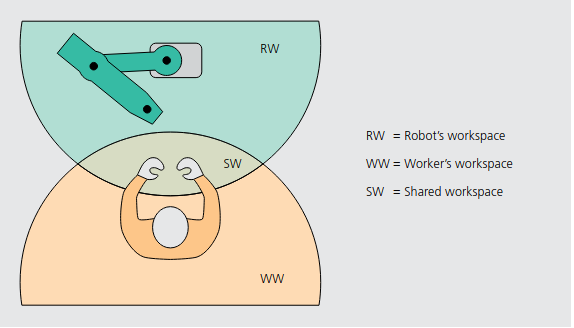
\includegraphics[width=0.8\textwidth]{workspaces}  % filename without extension
    \caption{Caption text.}
    \label{fig:Human, robot, and shared workspace from Fraunhofer \cite{benderLightweightRobotsManual2016}}
\end{figure}

Human--robot cooperation generally refers to the use of robots without safety fencing, also called cage--free robots. This in contrast to traditional robots which are stiff, heavy, and lack safety features that allow them to safely operate in the same space as humans, and are consequently only allowed to operate in closed of workspaces.

Human and robot can work together in different types of operation, stated below in figure x.

\begin{figure}[htbp]
    \centering
    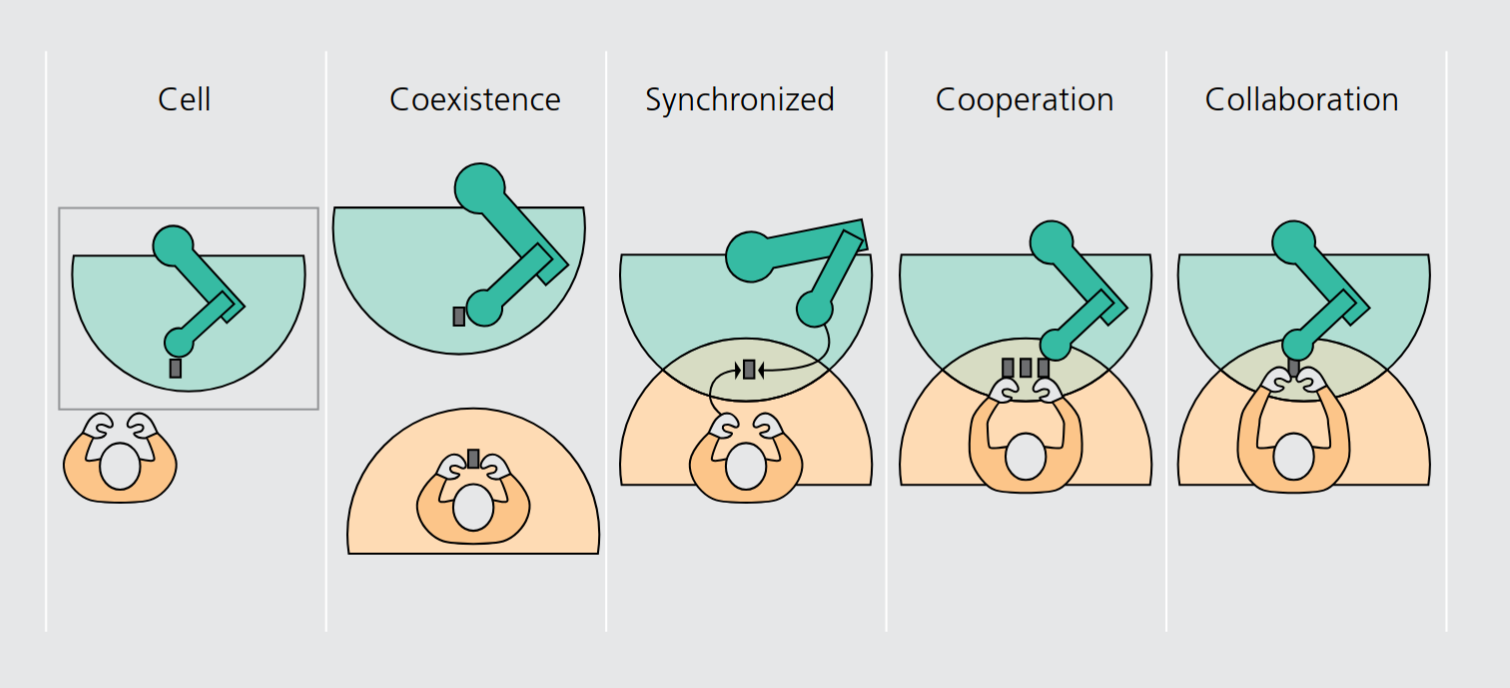
\includegraphics[width=0.8\textwidth]{Human_robot_collaboration}  % filename without extension
    \caption{Caption text.}
    \label{fig: Levels of cooperation between human worker and robot
    \cite{benderLightweightRobotsManual2016}}
\end{figure}

From left to right an increasing level of cooperation is shown. When robots operate in a cell, they are caged--off and there is no contact between human and robot. In a coexistent 
\vspace{0.2cm} 
\begin{itemize}[noitemsep, topsep=0pt]
	\item Safety--rated monitored stop
	\item Hand--guiding
	\item Power and force limiting
	\item Speed and separation monitoring
\end{itemize}
\vspace{0.3cm}



However, few collaborative applications currently exist in production facilities. In many cases, humans and robots are either physically separated or operate in a coexistence arrangement where no physical barrier exists, but no direct interaction takes place. Such implementations are only economically viable for large batch sizes, since a whole production line needs to be tuned towards that specific robotic solution.

Cage–-free robotic arms that share a workspace with a human worker are introduced to increase production flexibility. Interactive robotic solutions for small batches and varying product sizes has become a clear need since 70\% of collaboration between human worker and robotic solutions are found in assembly applications. An industry survey reported that 86\% of respondents were willing to invest in robotic solutions, indicating strong industrial interest. The primary motivations for introducing robotic arms in assembly environments are:
\vspace{0.2cm} 
\begin{itemize}[noitemsep, topsep=0pt]
	\item Improving operational efficiency
	\item Improving ergonomics
\end{itemize}
\vspace{0.3cm}

Cage–free robotic solutions generally involve higher initial costs compared to traditional fenced systems due to safety certification requirements and conformity procedures. Companies are however often willing to accept longer payback periods for implementing and testing company specific robotic solutions which increase ergonomics. Traditional stiff robots in collaborative applications are heavily regulated to minimize the risk
of injuries. These robots are lightweight, operate at low speeds and often lack mechanical bandwidth to react to unforeseen collisions in a safe and compliant way\cite{benderLightweightRobotsManual2016}.

One of the categorized modes of human robot collaboration (HRC) is hand-guiding, and is a potential solution for safe collaboration between human and robot. Hand–guided robotic applications are defined as a direct physical interaction between human and robot, where the human operator has full control over the robot motion. In this approach, a direct input device is located at or near the end–effector to measure input forces and simultaneously define the position of the human in the shared workspace. A direct consequence of this approach is that robotic applications with sensorised end–effectors can only react in a passive compliant manner when handled at a specific point on the robotic arm. Collisions or attemted handling of the robotic arm elsewhere will result in a safety stop of the robotic arm\cite{sicilianoSpringerHandbookRobotics2016a}.

Existing robotic solutions that allow a human worker to hand–guide a robotic arm by grasping it wherever is most convenient are, to the best of the authors' knowledge, practically non-existent in assembly and packaging industries. When hand–guiding is discussed in literature, it is typically limited to sensorised end–effectors on conventional stiff robots\cite{gregorHandGuidingVirtual2021}\cite{hameedControlSystemDesign2023}.

This absence in current industrial applications is further supported by surveys of end users, system integrators and researchers, which indicate that collaborative robots are still primarily implemented as traditional stiff robots with limited or no direct human interaction \cite{montiniCollaborativeRoboticsSurvey2024}.

\smalltitle{Example bold paragraph title}
Your text here \cite{somekey}.  % example citation

\begin{figure}[htbp]
    \centering
    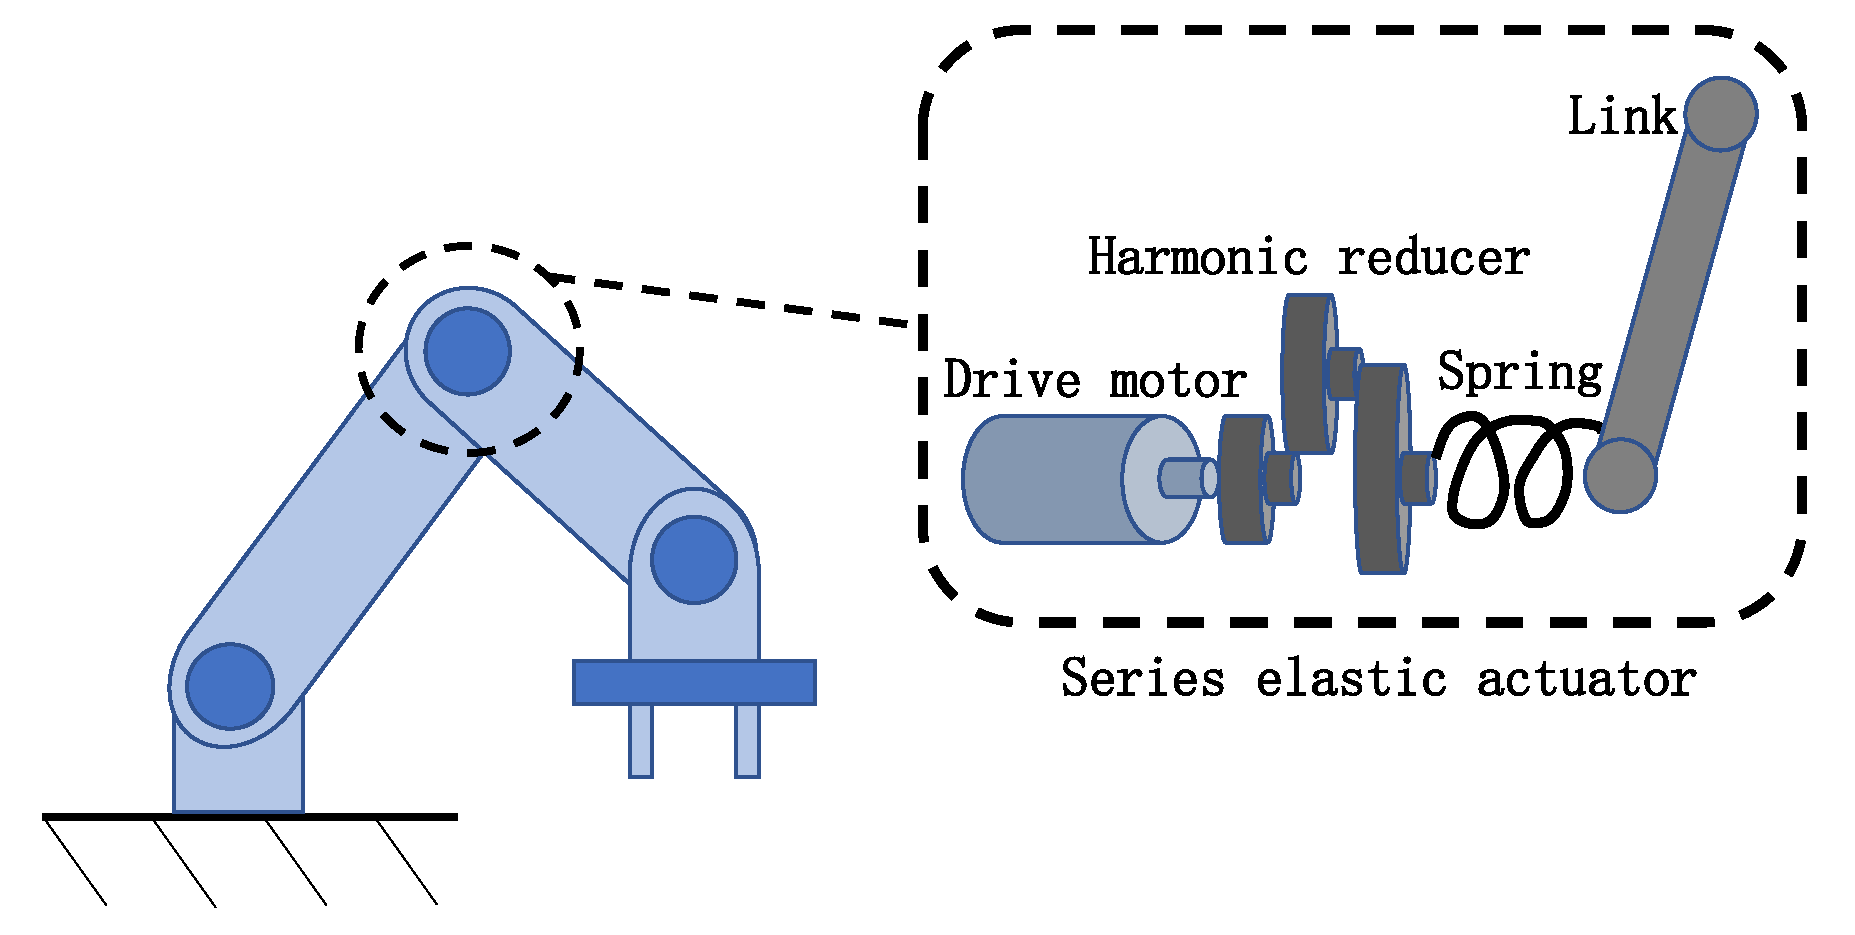
\includegraphics[width=0.8\textwidth]{SEA_Schematic}  % filename without extension
    \caption{Caption text.}
    \label{fig:example}
\end{figure}

\section{Problem Statement}
\label{sec:problem_statement}

\section{Thesis Outline}


% ============================================================
\chapter{Literature Review}
\label{ch:literature}
% ============================================================

\section{Theoretical Background}

\subsection{Example subsection}

Example equation:
\begin{equation}
    \tau = K_s \, \theta_s
    \label{eq:spring}
\end{equation}

\subsection{Another subsection}

\section{State of the Art}

\section{Gap Analysis}


% ============================================================
\chapter{System Design and Implementation}
\label{ch:design}
% ============================================================

\section{System Overview and Requirements}

\section{Mechanical Design}

\section{Hardware Architecture}

\subsection{CAN Bus Topology}

\subsection{Sensor Architecture}

\section{Sensor and Actuator Modelling}

\subsection{SET Spring Model}

\subsection{Motor and Transmission Model}

\section{Control Architecture}

\subsection{State Machine}

\subsection{Gravity Compensation and Floating Mode}

\subsection{Weighing Mode}

\subsection{Carrying Mode}

\subsection{Put-Down Mode}

\section{Software Implementation}

\subsection{Real-Time Architecture}

Example code listing:
\begin{lstlisting}[language=C++, caption={Example listing.}, label={lst:example}]
while (running) {
    clock_nanosleep(...);
    // your code here
}
\end{lstlisting}

\subsection{Configuration}


% ============================================================
\chapter{Validation and Results}
\label{ch:validation}
% ============================================================

\section{Experimental Setup}

\subsection{Hardware Configuration}

\subsection{Parameter Identification}

\section{Spring and Sensor Characterisation}

\section{Controller Performance}

\section{Assisted Load Handling Evaluation}

\section{Discussion}

Example table:
\begin{table}[htbp]
    \centering
    \caption{Example results table.}
    \label{tab:example}
    \begin{tabular}{@{}lcc@{}}
        \toprule
        Metric  & Target  & Achieved \\
        \midrule
        Value 1 & X       & Y        \\
        Value 2 & X       & Y        \\
        \bottomrule
    \end{tabular}
\end{table}


% ============================================================
\chapter{Conclusion and Future Work}
\label{ch:conclusion}
% ============================================================

\section{Conclusion}

\section{Future Work}


% ============================================================
%  BACK MATTER
% ============================================================
\backmatter

\printbibliography[heading=bibintoc, title={References}]

\appendix

\chapter{2D Manufacturing Drawings}
\label{app:drawings}

\section{CNC Part 1}
\section{CNC Part 2}
\section{CNC Part 3}

\chapter{Additional Experimental Results}
\label{app:results}

\chapter{Source Code}
\label{app:code}
\url{https://github.com/username/repository}   % <-- update

\end{document}